\documentclass[11pt]{article}

%PACKAGES
\usepackage{fxcm_format}
\usepackage{amsmath}
\usepackage{amssymb}
\usepackage{geometry}
\usepackage{minted}
\usepackage[most]{tcolorbox}

\definecolor{bgcolor}{RGB}{240, 240, 240} % Light gray background

\newtcolorbox{codebox}{
    breakable,
    colback=bgcolor, colframe=black,
    title=Sample Code, fonttitle=\bfseries,
    boxrule=1pt, arc=4pt, left=5pt, right=5pt, top=5pt, bottom=5pt
}

%\usepackage{draftwatermark}


%PROJECT INFORMATION
\newcommand{\project}{OAUTH Integration Guide}
\title{\project}
\author{Joe Harari}
\newcommand{\version}{Version 1.5}


%WATERMARK

% \SetWatermarkText{DRAFT}
% \SetWatermarkScale{1}
% \SetWatermarkColor[gray]{0.9}
 
%-------------------------FRONT PAGE------------------------
\title{\project}
\begin{document}
\maketitle
\vfill
\begin{center}
    
\includegraphics[width=0.9\textwidth]{tradufxcm.png}
\end{center}

\clearpage
%-------------------------END FRONT PAGE------------------------

\tableofcontents

\newpage

\section{Document Change Control}
 
\subsection{Document History}
\begin{tabular}{p{0.08\textwidth}p{0.50\textwidth}p{0.13\textwidth}p{0.15\textwidth}}\toprule
Version	& Change Description	&Author	&Date \\ \midrule
1.0 & 	Initial Document Creation	& Joe Harari & 22/11/2024\\
1.1 & 	Added "code" as a required parameter in the Body of Auth0 Access\_Token request. Added headers information for Auth0.	& Joe Harari & 27/11/2024\\
1.2 & Changed the Auth0 headers only for POST calls & Joe Harari & 02/12/2024 \\
1.3 & Added "audience" parameter to Auth0 Authorize Call & Joe Harari & 10/12/2024 \\
1.4 & Added section Conceptual Flow under Tradu & Joe Harari & 28/01/2024 \\
1.5 & Added code samples for every function & Joe Harari & 29/01/2024 \\


\bottomrule
\end{tabular}


 

 
\subsection{Document Approvers/Reviewers}
 
\begin{tabular}{p{0.3\textwidth}p{0.3\textwidth}p{0.3\textwidth}} \toprule
\textbf{Role}&\textbf{Name}& \textbf{Review Date} \\ \midrule
Gehtsoft  & Georgiy Golovin & 29/11/2024\\
\bottomrule
\end{tabular}		

 
\subsection{Document References}

\begin{itemize}
    \item \href{https://www.tradingview.com/broker-api-docs/trading/authentication/#oauth2-code-flow}{TradingView Oauth2 Code Flow}
    \item \href{https://auth0.com/docs/get-started/authentication-and-authorization-flow/authorization-code-flow}{Auth0 Authorization Code Flow}
    \item \href{https://github.com/fxcm/3rd-party-oauth}{FXCM 3rd Party OAUTH docs}
\end{itemize}

\newpage

% \newpage
\section{Introduction}
The purpose of this document is to describe the functionality and workflow of both FXCM's and Tradu's 3rd Party OAUTH authentication. 

\subsection{FXCM}

FXCM offers native OAUTH support in the shape of a custom-built OAUTH service following OAUTH2 principles. Crucially, since this service is custom-built, it allows users to login (via OAUTH) with simple CFD username/password combo.

FXCM’s Forex Connect Lite API requires a JWT to be passed in order to authenticate an end user and establish a trading session.  The 3rd party OAUTH authentication model allows a 3rd party application to direct the end user to FXCM’s authentication page.  

Upon successful authentication, FXCM will redirect back to the 3rd party application and provide the token.  This model follows standard OAUTH2 protocol and requires each 3rd party to register their callback URL with FXCM and get issued a \verb|client_id| and \verb|client_secret|.

\subsection{Tradu}

Tradu uses a different principle - Auth0 exists at the top and handles all authentication, and then every "silo" or component of the system can effectively rely on Auth0 for all auth needs.

This however poses an issue, in that Tradu \textit{cannot} use the same custom-built OAUTH service that FXCM uses, because Tradu customers do not use their CFD username/password (they don't even know it in fact). They use their Auth0 username/password instead, and our CFD system acknowledges Tokens generated using those credentials.

Tradu’s traduAPI API requires a JWT to be passed in order to authenticate an end user and establish a trading session.  The 3rd party OAUTH authentication model allows a 3rd party application to direct the end user to Auth0’s authentication page.  

Upon successful authentication, Auth0 will redirect back to the 3rd party application and provide the token. This model follows standard OAUTH2 protocol and requires each 3rd party to register their callback URL with FXCM and get issued a \verb|client_id| and \verb|client_secret|.

\subsection{Samples}
In both Tradu and FXCM, it is required by the partner or vendor to contact Tradu/FXCM and request access. 

We will create a client\_id and a client\_secret, as well as provide support/sample implementations of the OAUTH flow for ease of development.

\newpage
\section{Tradu OAUTH}

The integration in Tradu utilizes OAuth2 Code Flow for user authorization, as detailed in the documentation \href{https://auth0.com/docs/get-started/authentication-and-authorization-flow/authorization-code-flow}{here} and \href{https://www.tradingview.com/broker-api-docs/trading/authentication/#oauth2-code-flow}{here}

\subsection{Conceptual Flow}
The Auth0 OAuth flow being implemented is an \textbf{Authorization Code Grant flow with Refresh Tokens}. This flow is used for securely obtaining and refreshing access tokens for user authentication and authorization in third-party services. Below is a detailed breakdown of the steps.

\subsubsection*{1. \textbf{Initiating Authorization Request}}
\begin{itemize}
    \item \textbf{Action:} The user clicks the \textit{Sign In} button on the client application.
    \item \textbf{Request:} The client (browser) sends a \textbf{GET /authorize} request to the backend server.
    \item \textbf{Backend Behavior:}
          \begin{itemize}
              \item The backend server constructs an authorization URL for Auth0's `/authorize` endpoint
              \item The URL includes the following query parameters:
              \begin{itemize}
                  \item \textbf{response\_type:} \texttt{code} (indicates we want an authorization code).
                  \item \textbf{client\_id:} The public Client ID assigned for that specific application in Auth0. This value is specific to each application, and each environment.
                  \item \textbf{redirect\_uri:} URL to redirect the user back to after successful authentication (e.g., \texttt{http://localhost:3000/authorized} or whatever other URL the application wants the client to be returned to).
                  \item \textbf{scope:} Requested permissions (e.g., \texttt{openid profile offline\_access}).
                   \item \textbf{audience:} This tells Auth0 which audience this application wants to authenticate into, based on the permissions it has configured
                  \item \textbf{state:} A random string to mitigate CSRF attacks.
              \end{itemize}
              \item The backend redirects the user to the constructed authorization URL.
          \end{itemize}
    \item \textbf{Result:} The user's browser is redirected to Auth0's login page for authentication.
\end{itemize}

\subsubsection*{2. \textbf{User Authentication (on Auth0)}}
\begin{itemize}
    \item \textbf{Action:} The user authenticates with their credentials (e.g., username/password or social login) on Auth0's hosted login page.
    \item \textbf{Result:} Auth0 verifies the user's credentials and, if valid, redirects the user back to the \texttt{redirect\_uri} specified earlier, with an \textbf{authorization code} in the query string.
\end{itemize}

\subsubsection*{3. \textbf{Authorization Code Exchange}}
\begin{itemize}
    \item \textbf{Request:} The backend server receives the authorization code at the \texttt{/authorized} endpoint via a GET request:
    \[
    \text{GET /authorized?code=<authorization\_code>&state=<state>}
    \]
    \item \textbf{Backend Behavior:}
          \begin{itemize}
              \item The backend verifies the \texttt{state} parameter to ensure the request is legitimate.
              \item The backend sends a \textbf{POST} request to Auth0's \texttt{/oauth/token} endpoint to exchange the authorization code for tokens. The request body includes:
              \begin{itemize}
                  \item \textbf{grant\_type:} \texttt{authorization\_code}.
                  \item \textbf{code:} The authorization code received from Auth0.
                  \item \textbf{redirect\_uri:} Must match the original redirect URI from Step 1.
                  \item \textbf{client\_id:} The Client ID from Auth0.
                  \item \textbf{client\_secret:} The Client Secret from Auth0.
              \end{itemize}
          \end{itemize}
    \item \textbf{Result:} Auth0 responds with a JSON payload containing:
          \begin{itemize}
              \item \textbf{access\_token:} Token used to access protected resources.
              \item \textbf{id\_token:} Token containing user information (e.g., claims like name, email, etc.).
              \item \textbf{refresh\_token:} Token used to request new access tokens when the current one expires.
          \end{itemize}
\end{itemize}

\subsubsection*{4. \textbf{Accessing Protected Resources}}

The way Access Token is implemented in the Tradu system is different from
other brokers. Tradu is a state\textit{full} stack, not a state\textit{less} stack. Meaning that an Access Token is only needed once, to create a Trading Session with the system. 

Once a Trading Session has been established, new Access Tokens are not required and customers
are free to trade.

Once a trading session dies due to any reason - session killed by Tradu middleware,
session killed by user’s browser, session killed by partner - when client wants to jump
back into the platform, a new Access Token must be fetched via Refresh mechanism,
and a new Trading Session must be created using that token.

In effect, the Access Token is a simple key that allows you to start a Trading Session -
once the session has been created, you no longer need it. It is not a Bearer Token.

\begin{itemize}
    \item \textbf{Action:} The backend stores the \textbf{access token}, \textbf{id token}, and \textbf{refresh token} in the user's session.
    \item \textbf{Result:} The user is redirected to the home page or another protected resource.
\end{itemize}

\subsubsection*{5. \textbf{Refreshing Tokens (Optional)}}
\begin{itemize}
    \item \textbf{Request:} When the access token expires, the client can request a new one by sending a \textbf{POST} request to Auth0's \texttt{/oauth/token} endpoint. The request body includes:
          \begin{itemize}
              \item \textbf{grant\_type:} \texttt{refresh\_token}.
              \item \textbf{refresh\_token:} The refresh token stored in the session.
              \item \textbf{client\_id:} The Client ID from Auth0.
              \item \textbf{client\_secret:} The Client Secret from Auth0.
          \end{itemize}
    \item \textbf{Result:} Auth0 responds with a new \textbf{access token} (and optionally a new refresh token).
\end{itemize}

\subsubsection*{6. \textbf{Logging Out}}
\begin{itemize}
    \item \textbf{Request:} When the user logs out, the backend redirects them to Auth0's \texttt{/oidc/logout} endpoint with the following parameters:
          \begin{itemize}
              \item \textbf{id\_token\_hint:} The current ID token, to inform Auth0 which session to end.
              \item \textbf{post\_logout\_redirect\_uri:} URL to redirect the user after logging out.
          \end{itemize}
    \item \textbf{Result:} Auth0 clears the session and redirects the user to the specified URL.
\end{itemize}

\subsubsection*{Summary of Data Points}
\begin{itemize}
    \item \textbf{Initial Authorization Request:}
          \begin{itemize}
              \item Required: \texttt{client\_id}, \texttt{redirect\_uri}, \texttt{scope}, \texttt{audience}.
              \item Result: Authorization Code.
          \end{itemize}
    \item \textbf{Token Exchange:}
          \begin{itemize}
              \item Required: \texttt{client\_id}, \texttt{client\_secret}, \texttt{redirect\_uri}, \texttt{code}.
              \item Result: \texttt{access\_token}, \texttt{id\_token}, \texttt{refresh\_token}.
          \end{itemize}
    \item \textbf{Refresh Tokens:}
          \begin{itemize}
              \item Required: \texttt{client\_id}, \texttt{client\_secret}, \texttt{refresh\_token}.
              \item Result: New \texttt{access\_token}.
          \end{itemize}
\end{itemize}


\subsection{Gathering Information/Set-Up on Tradu's side}

To configure the Auth0 application for any third-party integration, we will need the following information from the vendor:

\begin{itemize}
    \item Allowed Callback URL
    \item Allowed Logout URL
    \item Technology stack (Java, Node.js, etc.)
\end{itemize}

Additionally, it’s important to confirm the following points with the partner in question

\begin{itemize}
    \item As stated \href{https://auth0.com/docs/api/authentication#refresh-token}{here}, Auth0 requires the \verb|client_id| field to be included in all refresh token requests.
    \item The partner must have policies in place that automatically closes the authorization window on the Tradu side if the user remains inactive for a specified period.
\end{itemize}

We will follow these steps to set up the new application in Auth0:

\begin{itemize}
    \item Application Type: Create a new application of type Regular Web Application and specify the technology stack used by the partner.
    \item Custom Domain: Confirm that the Auth0 tenant is configured with a custom domain.
    \item Settings Tab Configuration:
    \begin{itemize}
        \item Define Allowed Callback URL and Allowed Logout URLs (consult partner for exact URLs).
    \end{itemize}
    \item Token Settings:
    \begin{itemize}
        \item In the Refresh Token Rotation section, enable "Allow refresh token rotation".
    \end{itemize}
    \begin{itemize}
        \item Configure token lifetimes to ensure that the refresh token has a longer lifetime than the access token, facilitating successful token renewal.
    \end{itemize}
    \item Advanced Settings:
    \begin{itemize}
        \item OAuth Tab: Ensure that OIDC Conformant is enabled.
    \end{itemize}
    \begin{itemize}
        \item Grant Types Tab: Confirm that both Authorization Code and Refresh Token grant types are enabled.
    \end{itemize}
\end{itemize}

An AWS ticket must be logged in order for this setup (Example AWS-456)

\subsection{Integration Setup on the Partner's side}

\begin{figure}[H]
    \centering
    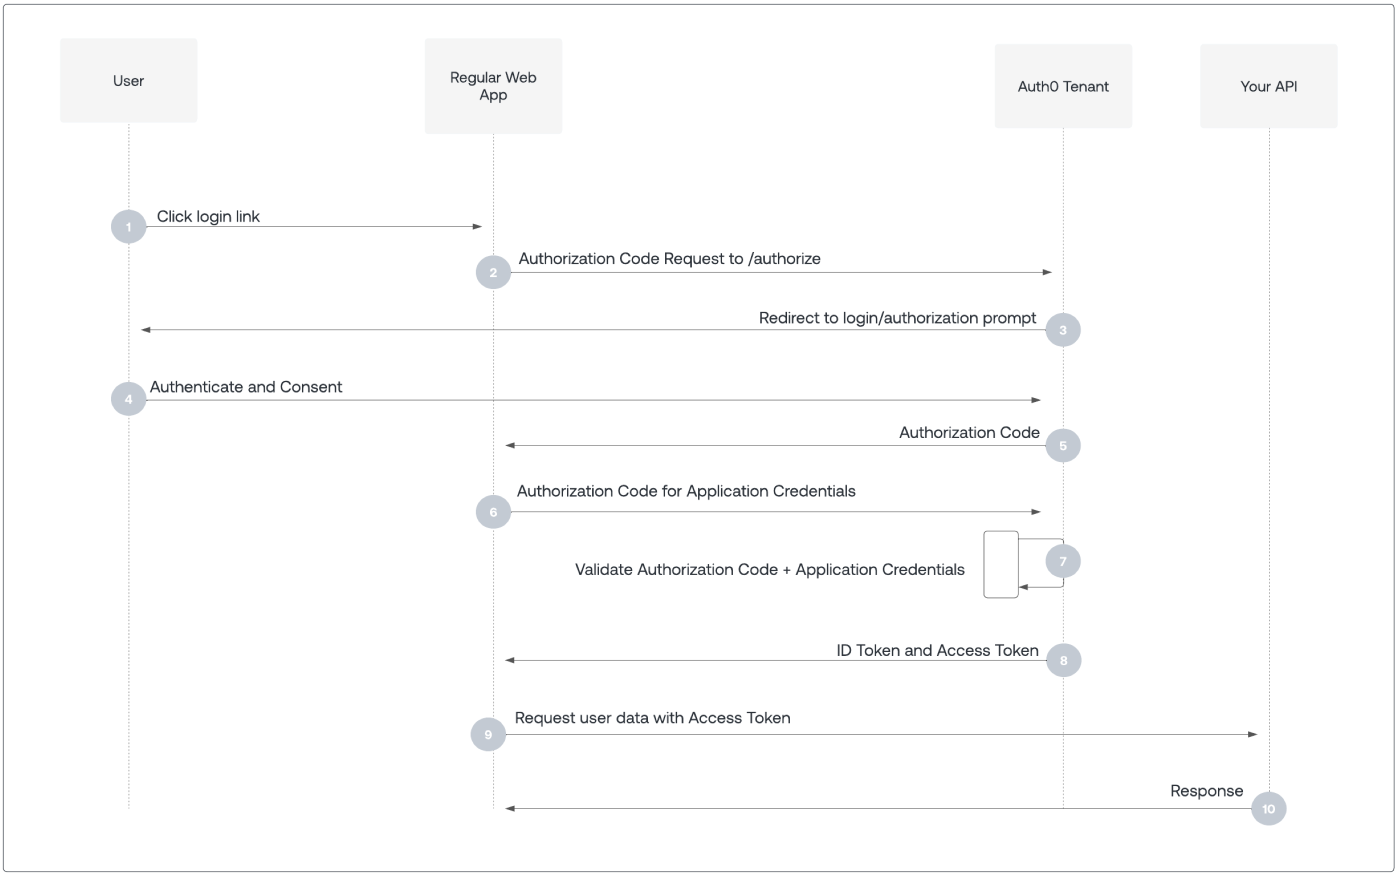
\includegraphics[width=1.0\linewidth]{Auth-code-flow-diagram.png}
    \caption{Caption}
    \label{Auth0 Code Flow}
\end{figure}

All Tradu URLs are of the form \url{https://authx.tradu.com} where "x" is a variable that denotes the environment

\begin{itemize}
    \item authd denotes "Dev"
    \item authu denotes "UAT"
    \item auth denotes "Production"
\end{itemize}

These are completely different and separate environments - logins that work in authd will not work in authu and viceversa

\paragraph{Authorize URL}

\begin{verbatim}
GET
https://authx.tradu.com/oauth/authorize?
response_type=code
&scope=openid%20profile%20offline_access
&audience=http%3A%2F%2Faccount-portal%2Fapi
&client_id=[client_id]
&redirect_uri=[redirect_uri]
&state=[state]
\end{verbatim}

Where

\begin{itemize}
    \item \verb|x|: the environment in question (d, u, or blank) 
    \item \verb|response_type|: always \verb|code|
    \item \verb|scope|: always \verb|openid profile offline_access|
    \item \verb|audience|: to access CFD accounts, always \verb|http://account-portal/api|
    \item \verb|client_id|: Will be provided by Tradu
    \item \verb|redirect_uri|: Must match the URL configured in the system
     \item \verb|state|: Optional opaque value set by the client which the authorisation server will echo verbatim in the authorisation response. Enables the client to encode application state information to appear at the \verb|redirect_uri|.
\end{itemize}

Returns \verb|code| as query parameter

\begin{codebox}
\begin{minted}[fontsize=\small, breaklines]{javascript}
// GET /authorize endpoint
app.get('/authorize', (req, res) => {
    console.log('[DEBUG] Processing /authorize request...');

    const url = new URL(CONFIG.oauth_url);
    const clientId = CONFIG.client_id;
    const redirectURL = CONFIG.redirect_url;

    url.pathname = '/oauth/authorize';
    url.searchParams.set('response_type', 'code');
    url.searchParams.set('scope', 'openid profile offline_access');
    url.searchParams.set('client_id', clientId);
    url.searchParams.set('redirect_uri', redirectURL);
    url.searchParams.set('audience', 'http://account-portal/api');

    console.log('[DEBUG] Redirecting to:', url.toString());
    res.redirect(url.toString());
});
\end{minted}
\end{codebox}


\paragraph{Access Token URL}

\begin{verbatim}
POST
https://authx.tradu.com/oauth/token
\end{verbatim} 

With headers

\begin{verbatim}
    headers: {'content-type': 'application/x-www-form-urlencoded'},
\end{verbatim}

With body

\begin{verbatim}
    {
      'client_id': '',
      'client_secret': '',
      'grant_type': 'authorization_code',
      'redirect_uri': '',
      'code': ''
    },
\end{verbatim}


Where

\begin{itemize}
    \item \verb|x|: the environment in question (d, u, or blank) 
    \item \verb|client_id|: Will be provided by Tradu
    \item \verb|client_secret|: Will be provided by Tradu
    \item \verb|grant_type|: Always "authorization\_code"
    \item \verb|redirect_uri|: Must match the URL configured in the system.
    \item \verb|code|: The code returned by the Authorize call

\end{itemize}

\begin{codebox}
\begin{minted}[fontsize=\small, breaklines]{javascript}
// GET /authorized endpoint
app.get('/authorized', (req, res) => {
    console.log('Processing /authorized request...');
    if (req.query.error) {
        console.error('Authorization error:', req.query.error);
        res.json({ error: req.query.error });
        return;
    }

    console.log('Authorization code received:', req.query.code);

    const tokenURL = CONFIG.oauth_url + '/oauth/token';
    const postBody = {
        grant_type: 'authorization_code',
        redirect_uri: CONFIG.redirect_url,
        code: req.query.code,
        client_id: CONFIG.client_id,
        client_secret: CONFIG.client_secret,
    };

    console.log('Exchanging authorization code for tokens...');
    console.log('Token exchange request body:', postBody);

    axios
        .request({
            withCredentials: true,
            headers: { 'content-type': 'application/x-www-form-urlencoded' },
            method: 'POST',
            url: tokenURL,
            data: querystring.stringify(postBody),
        })
        .then((result) => {
            console.log('Token exchange response:', result.data);
            req.session.access_token = result.data.access_token;
            req.session.refresh_token = result.data.refresh_token || 'No refresh token';
            req.session.id_token = result.data.id_token;

            console.log('Session after token exchange:', {
                access_token: req.session.access_token,
                refresh_token: req.session.refresh_token,
                id_token: req.session.id_token,
            });

            res.redirect('/');
        })
        .catch((err) => {
            console.error('Token exchange error:', err.response?.data || err.message);
            res.redirect('/');
        });
});
\end{minted}
\end{codebox}

\paragraph{Logout URL}

\begin{verbatim}
GET
https://authx.tradu.com/oidc/logout?
post_logout_redirect_uri={redirect_uri}
&id_token_hint={id_token}
&client_id={client_id}
\end{verbatim}

Where

\begin{itemize}
    \item \verb|x|: the environment in question (d, u, or blank)
    \item \verb|client_id|: Will be provided by Tradu
    \item \verb|redirect_uri|: Must match the URL configured in the system
\end{itemize}

\begin{codebox}
\begin{minted}[fontsize=\small, breaklines]{javascript}
// GET /logout endpoint
app.get('/logout', (req, res) => {
    console.log('Processing /logout request...');
    const url = new URL(CONFIG.oauth_url);
    url.pathname = '/oidc/logout';

    url.searchParams.set('id_token_hint', req.session.id_token);
    url.searchParams.set('client_id', CONFIG.client_id);

    console.log('Redirecting to logout URL:', url.toString());
    req.session.destroy();
    res.redirect(url.toString());
});
\end{minted}
\end{codebox}

\paragraph{Token Refresh URL}
\begin{verbatim}
GET
https://authx.tradu.com/oauth/token?grant_type=refresh_token
&refresh_token={refresh_token}
&client_id={client_id}
&client_secret={client_secret}
\end{verbatim}

Where 

\begin{itemize}
    \item \verb|x|: the environment in question (d, u, or blank)
    \item \verb|refresh_token|: The Refresh Token
    \item \verb|client_id|: Will be provided by Tradu
    \item \verb|client_secret|: Will be provided by Tradu
\end{itemize}

\begin{codebox}
\begin{minted}[fontsize=\small, breaklines]{javascript}
// GET /refresh endpoint
app.get('/refresh', (req, res) => {
    console.log('Processing /refresh request...');
    if (!req.session.refresh_token) {
        console.error('No refresh token found in session.');
        res.json({ error: 'No refresh token' });
        return;
    }

    const tokenURL = CONFIG.oauth_url + '/oauth/token';
    const postBody = {
        grant_type: 'refresh_token',
        refresh_token: req.session.refresh_token,
        client_id: CONFIG.client_id,
        client_secret: CONFIG.client_secret,
    };

    console.log('Refresh token request body:', postBody);

    axios
        .request({
            withCredentials: true,
            headers: { 'content-type': 'application/x-www-form-urlencoded' },
            method: 'POST',
            url: tokenURL,
            data: querystring.stringify(postBody),
        })
        .then((result) => {
            console.log('Refresh token response:', result.data);
            req.session.access_token = result.data.access_token;
            req.session.refresh_token = result.data.refresh_token;

            console.log('Session after refresh token exchange:', {
                access_token: req.session.access_token,
                refresh_token: req.session.refresh_token,
            });

            res.redirect('/');
        })
        .catch((err) => {
            console.error('Refresh token error:', err.response?.data || err.message);
            res.redirect('/');
        });
});
\end{minted}
\end{codebox}
\paragraph{Accessing Protected Resources}
Partner must use the \href{https://docs.gehtsoftusa.com/tradu_api/core/core/classes/IFXConnectLiteSessionMethods/IFXConnectLiteSession.loginByExternalSsoToken.html}{LoginByExternalSSOToken} method in traduAPI in order to create a trading session.

\begin{table}[h]
    \centering
    \begin{tabular}{l l l}
        \toprule
        Environment & tradingSystemUrl & connection \\
        \midrule
        authd   & \verb|https://fxcorpmcx.fxcorporate.com| & \verb|QAMCCLANE| \\
        authu & \verb|https://fxcorpmcz.fxcorporate.com| & \verb|UATMC| \\
        auth & \verb|https://fxcorpmc.fxcorporate.com|  & \verb|RealMC| \\
        \bottomrule
    \end{tabular}
    \caption{Trading System Environments}
    \label{tab:trading_envs}
\end{table}

It is not possible to login with \verb|LoginByExternalSSOToken| to appq (QA environment)

Partner must ensure that the configuration is done correctly to the appropriate Auth0 environment.

For example: If partner is using https://authd.tradu.com/oauth/ to authenticate, when instantiating a session in TraduAPI and calling \verb|LoginByExternalSSOToken|, the following parameters must be set

\begin{itemize}
    \item \verb|https://fxcorpmcx.fxcorporate.com| as the tradingSystemUrl 
    \item \verb|QAMCCLANE| as the connection
\end{itemize}

\begin{codebox}
\begin{minted}[fontsize=\small, breaklines]{javascript}
import { FXConnectLiteSessionFactory } from '@gehtsoft/traduAPI-node';

const jwt = 'valid access_token';

(async function () {
    let session = FXConnectLiteSessionFactory.create('LoginSample');
    try {
        // Define a basic handler to avoid `undefined` errors
        // session.onLoginError = (error) => console.error('Login error:', error);
        
        const startTimeInMilliseconds = new Date().getTime();;
        await loginByExternalSsoToken(session, jwt, "https://fxcorpmcx.fxcorporate.com", "QAMCCLANE");

        if (session.getConnectionStatus().isConnected()) {
            const totalTimeInMilliseconds = new Date().getTime() - startTimeInMilliseconds;
            console.log(`Connection time in milliseconds: ${totalTimeInMilliseconds}`);
            console.log('Connected');
        }

        // Perform requests here

    } catch (ex) {
        console.error(ex);
        process.exit(1);
    } finally {
        if (session && session.getConnectionStatus().isConnected()) {
            await logout(session);
            if (session.getConnectionStatus().isDisconnected()) {
                console.log('Disconnected');
            }
        }
    }
})();

\end{minted}
\end{codebox}




\newpage
\section{FXCM OAUTH}

The integration in FXCM utilizes a custom-built authorization\_code grant type for user authorization, as detailed in the documentation \href{https://datatracker.ietf.org/doc/html/draft-ietf-oauth-v2-1-01}{here}.

\subsection{Gathering Information}

To configure the FXCM OAUTH2 application for any third-party integration, we will need the following information from the vendor:

\begin{itemize}
    \item Allowed Callback URL
    \item Allowed Logout URL
\end{itemize}


\subsection{Setting Up a New Application}
Setting up is quite simple - requires a simple PROD ticket requesting this. Example ticket PROD-7274.

PROD will configure the new application in the system, and provide four params: \verb|client_id|, \verb|client_secret|, \verb|redirect_uri| and \verb|logout_uri|.

These four params are necessary and should be provided to the partner.

\subsection{Integration Setup on the Partner's side}

Partner must launch the Authorize URL as specified in the URLs section

The end user must enter their FXCM login credentials. The user will be prompted to and must subsequently approve the request.

If the request is successful, the FXCM Auth Server will redirect back to \verb|redirect_uri| with the query parameter: \verb|code|, and the	3rd party application will receive response with header.location: \verb|redirect_uri?code={code}|

After this, the 3rd party application must submit a POST request to the Access Token URL as specified in the URLs section.

If the request is successful, the FXCM Auth Server will return a response of the following format:

\begin{verbatim}
{access_token: access_token, refresh_token: refresh_token, token_type: ‘Bearer’}
\end{verbatim}

Where

\begin{itemize}
    \item access\_token: a valid access token (usually valid for 1 minute) which can be used to create a session with FCLite
    \item refresh\_token: a refresh token which can be used to get a new access token (usually valid for 24 hours)
\end{itemize}

The 3rd party application may submit a POST to get new access token through the refresh mechanism specified in the URLs section

The 3rd party application may submit a POST to logout and clear cookies through the logout mechanism specified in the URLs section.

\subsection{URLs}
All FXCM URLs are of the form \url{https://oauthx.fxcorporate.com} where "x" is a variable that denotes the environment

\begin{itemize}
    \item oauthq denotes "QA"
    \item oauth-demo denotes "DEMO"
    \item oauth denotes "Production"
\end{itemize}

These are completely different and separate environments - logins that work in oauthq will not work in oauth-demo and viceversa

\paragraph{Authorize URL}

\begin{verbatim}
https://oauthx.fxcorporate.com/oauth/authorize?response\_type=code
&client_id=[client_id]
&redirect_uri=[redirect_uri]
&scope=openid\%20trading
\end{verbatim}

Where

\begin{itemize}
    \item \verb|x|: the environment in question (q, -demo, or blank) 
    \item \verb|client_id|: Will be provided by FXCM
    \item \verb|redirect_uri|: Must match the URL configured in the system
\end{itemize}

Optional parameters are as follows:

\begin{enumerate}
    \item code\_challenge\_method: Set to S256 to indicate that SHA-256 hashing is used to transform the code verifier.
    \item code\_challenge: The BASE64URL-encoded SHA-256 hash of a random 32 bytes called code verifier which the client must generate and store internally and which is intended to prevent code injection and CSRF attacks. Originally specified in the PKCE extension (RFC 7336) to OAuth 2.0.
    \item state: Optional opaque value set by the client which the authorisation server will echo verbatim in the authorisation response. Enables the client to encode application state information to appear at the \verb|redirect_uri|.
    \item nonce: String value used to associate a Client session with an ID Token, and to mitigate replay attacks. 
    \begin{itemize}
        \item The value is passed through unmodified from the Authentication Request to the ID Token. 
        \item If present in the ID Token, Clients MUST verify that the nonce Claim Value is equal to the value of the nonce parameter sent in the Authentication Request. 
        \item If present in the Authentication Request, Authorization Servers MUST include a nonce Claim in the ID Token with the Claim Value being the nonce value sent in the Authentication Request. \item Authorization Servers SHOULD perform no other processing on nonce values used. 
        \item The nonce value is a case sensitive string.
    \end{itemize}
\end{enumerate}

\paragraph{Access Token URL}

\begin{verbatim}
POST
https://oauthx.fxcorporate.com/oauth2/token
\end{verbatim} 

Where

\begin{itemize}
    \item \verb|x|: the environment in question (q, -demo or blank) 
    \item code: the code returned in the Authenticate request
    \item \verb|client_id|: Will be provided by FXCM
    \item \verb|client_secret|: Will be provided by FXCM
    \item \verb|grant\_type|: Always "authorization\_code"
    \item \verb|redirect_uri|: Must match the URL configured in the system
\end{itemize}

\paragraph{Logout URL}

\begin{verbatim}
POST
https://oauthx.fxcorporate.com/oauth2/logout 
\end{verbatim}

Where

\begin{itemize}
    \item \verb|x|: the environment in question (q, -demo, or blank)
    \item \verb|client_id|: Will be provided by Tradu
    \item \verb|redirect_uri|: Must match the URL configured in the system
\end{itemize}

\paragraph{Token Refresh URL}
\begin{verbatim}
POST
https://oauthx.fxcorporate.com/oauth2/token
\end{verbatim}

Where 

\begin{itemize}
    \item \verb|x|: the environment in question (q, -demo, or blank)
    \item refresh\_token: The Refresh Token
    \item \verb|client_id|: Will be provided by Tradu
    \item \verb|client_secret|: Will be provided by Tradu
    \item \verb|redirect_uri|: must match the URL configured in the system
    \item grant\_type: 'refresh\_token'
\end{itemize}



\end{document}